\subsection{限制对偶与矩阵系数}

命题 3. —— 设 \((\mathrm{V},\pi)\) 是代数 A 的一个有限维线性表示。核 \(\mathfrak{a}\)（即 \(\pi\) 的核）是 A 的一个有限余维数双边理想，且 \(\Theta_{\pi}(\mathrm{A})\) 是 \(\mathfrak{a}\) 在 \(A^{*}\) 中的正交。映射 \(\pi\) 的转置定义了从 K-向量空间 \(\pi(\mathrm{A})\) 的对偶到 \(\Theta_{\pi}(\mathrm{A})\) 的一个同构。

由于 \(\operatorname{End}_{\mathrm{K}}(\mathrm{V})\) 在 K 上有限维，\(\mathfrak{a}\) 是 A 的一个有限余维数双边理想。向量空间 \(\Theta_{\pi}(\mathrm{A})\) 是 \(A^{*}\) 的一个有限维子空间，它在 A 中的正交等于 \(\mathfrak{a}\)；由 II, §7, No.~5, 第 301 页，定理 7，空间 \(\Theta_{\pi}(\mathrm{A})\) 因而是 \(\mathfrak{a}\) 在 \(A^{*}\) 中的正交。此外，由于 \(\mathfrak{a}\) 是 \(\pi\) 的核，映射 \(\pi\) 的转置定义了从 \(\pi(\mathrm{A})\) 的对偶到 \(\mathfrak{a}\) 在 \(A^{*}\) 中的正交的一个同构（II, §7, No.~5, 第 299 页，定理 5 的推论）。

推论. —— A 的限制对偶 \(\Theta(\mathrm{A})\) 是 A 的有限维线性表示的系数所成的集。

按定义，\(\Theta(A)\) 是 \(A\) 的有限余维数双边理想的正交的并。因此我们有 \(\Theta_{\pi}(A) \subset \Theta(A)\)（\(\pi\) 为 \(A\) 的任意一个有限维线性表示）。反之，设 \(f\) 是 \(\Theta(A)\) 的一个元素，\(\mathfrak{a}\) 是一个包含在 \(f\) 的核中的有限余维数双边理想（VIII, 第 376 页，定义 2）。用 \(\pi\) 表示 \(A\) 在 \(A/\mathfrak{a}\) 中的、由 \(A\) 中的左正则表示通过过渡到商而得到的线性表示。设 \(x\) 是 1 的类（模 \(\mathfrak{a}\)），\(x^{*}\) 是 \(A/\mathfrak{a}\) 上的、由 \(f\) 得到的线性形式。我们有 \(f = c_{\pi}(x, x^{*})\)，故 \(f\) 是 \(\pi\) 的一个系数。

\pandocbounded{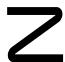
\includegraphics[keepaspectratio]{images/part003_35b408b4.jpg}}

注意：若 \((V,\pi)\) 是 A 的一个在 K 上非有限维的线性表示，则空间 \(\Theta_{\pi}(A)\) 未必包含在 \(\Theta(A)\) 中。

